$\bm{Z} = R\bm{V}$, where $\bm{V} \in \mathbb{S}_{\infty}^{d-1}$; 
$R \in \mathbb{R}_+$; $R$ and $\bm{V}$ are independent.  
$\bm{Y} = T_p(\bm{V})$ is the normalization of $\bm{V}$ onto 
$\mathbb{S}_p^{d-1}$.

\subsection{Target Distribution (gamma prior)}
\begin{equation}
    \begin{aligned}
        \bm{y}_i \mid \bm{\alpha}_i &\sim
        \mathcal{PG}_p\left(\bm{Y}\mid\bm{\alpha}_i,\bm{1}\right)\\
        \bm{\alpha}_i &\sim G\\
        G &\sim \mathcal{PY}\left(\eta, d, G_0\right)        
    \end{aligned}
    ~\hspace{1cm}
    \begin{aligned}
        G_0 &= {\textstyle\prod}_{\ell = 1}^{d}\mathcal{G}(\alpha_{\ell}\mid \xi_{\ell},\tau_{\ell})\\
        \xi_{\ell} &\sim \mathcal{G}(\xi\mid a, b)\\
        \tau_{\ell} &\sim \mathcal{G}(\tau\mid c, d)
    \end{aligned} 
\end{equation}
If we expand the Pitman--Yor process using stick-breaking notation with truncation point $J$, we can write the above as
\begin{equation}
    \begin{aligned}
        \nu_j\mid\eta &\sim \mathcal{B}(1 - d, \eta + kd)\\
        \bm{\pi} &= \pi(\bm{\pi})\\
        \alpha_{j\ell} &\sim \mathcal{G}(\alpha\mid\xi_{\ell},\tau_{\ell})
    \end{aligned}
    ~\hspace{1cm}
    \begin{aligned}
        \xi_{\ell} &\sim \mathcal{G}(\xi \mid a, b)\\
        \tau_{\ell} &\sim \mathcal{G}(\tau\mid c, d)\\
        \bm{y}_i \mid \ldots &\sim {\textstyle\sum}_{j = 1}^Jw_i\mathcal{PG}(\bm{y}\mid\bm{\alpha}_j, \bm{1})
    \end{aligned}   
\end{equation}
where $\pi(\bm{\nu})$ is a function of $\bm{\nu}$ such that
\begin{equation*}
    \bm{\pi} = \pi(\bm{v}) = \begin{cases}
        \nu_j &\text{ for }j = 1\\
        \nu_j{\textstyle\prod}_{k < j}(1 - \nu_k) &\text{ for }j = 2,\ldots,J-1\\
        {\textstyle\prod}_{k < j}(1 - \nu_k) &\text{ for }j = J
    \end{cases}
\end{equation*}
Fitting the above model is accomplished using a variational approximation.  As a first pass, we attempt a simple surrogate posterior using a mean field representation.

\subsubsection{Gaussian Mean Field Variational Family surrogate posterior for Pitman-Yor mixture of projected gammas, gamma prior}
The mean field surrogate posterior creates an independent distribution for every parameter of the model, ideally with the appropriate transformation
for each parameter such that the support of the transformed variable is the real line.   Optimization through gradient ascent makes discrete parameters ineligible
for fitting through a variational approach, so we ascertain cluster weights globally rather than sampling the underlying cluster membership.
\begin{equation}
    \begin{aligned}
    \bm{\nu} &\sim {\textstyle\prod}_{j = 1}^J\text{Logit}\mathcal{N}(\nu_j\mid\mu_{\nu_j},\sigma^2_{\nu_j})\\
    \bm{\alpha} &\sim {\textstyle\prod}_{j = 1}^J{\textstyle\prod}_{\ell = 1}^D\mathcal{LN}(\alpha_{j\ell}\mid\mu_{\alpha_{j\ell}},\sigma^2_{\alpha_{j\ell}})
    \end{aligned}
    ~\hspace{1cm}
    \begin{aligned}
    \bm{\xi} &\sim{\textstyle\prod}_{\ell = 1}^D\mathcal{LN}(\xi_{\ell}\mid\mu_{\xi_{\ell}},\sigma^2_{\xi_{\ell}})\\
    \bm{\tau} &\sim{\textstyle\prod}_{\ell = 1}^D\mathcal{LN}(\tau_{\ell}\mid\mu_{\tau_{\ell}}, \sigma^2_{\tau_{\ell}})
    \end{aligned}
\end{equation}
We fit this surrogate posterior in \emph{tensorflow} using automatic differentiation to calculate the gradient, and 

\subsection{Variational Approximation with exact sampling}
This variational approximation makes use of the exact sampling of latent variables as detailed in \cite{Loaizamaya2022} to
sample cluster membership, and thus cluster weights, via their full conditional distributions.  Then, conditional on
the sampled cluster weights/memberships, a simpler variational approximation is available for cluster and prior parameters.

Under the stick-breaking representation, cluster membership is distributed categorically as
\begin{equation}
    \text{P}(\gamma_i = j) \propto \pi_j\mathcal{PG}(\bm{y}_i\mid\bm{\alpha}_j,\bm{1})
\end{equation}
with the appropriate normalizing constant.  Then, the raw cluster weight $\nu_j$ is distributed as
\begin{equation}
    \nu_j\mid\bm{\gamma} \sim \text{Beta}(\eta - d + n_j,1 + jd + \sum_{k > j}n_k)
\end{equation}
where $n_j = \sum_{i:\gamma_i = j}1$.  Then $\bm{\pi} = \pi(\bm{\nu})$.

Let $\theta = (\bm{\alpha},\bm{\xi},\bm{\tau})$ be a subset of parameters for which the distribution will be approximated via variational inference,
and $\phi = (\bm{\gamma},\bm{\nu})$ be the latent parameters that will be sampled via their full conditional distributions.  Then,
\begin{equation}
    \begin{aligned}
        f(\bm{y},\theta\mid\phi) &\propto \mathcal \prod_{j = 1}^J\left[\prod_{i:\gamma_i = j}\left[\mathcal{PG}(\bm{y}_i\mid\bm{\alpha}_j,\bm{1})\right]\times\prod_{\ell = 1}^d\mathcal{G}(\alpha_{j\ell}\mid\xi_{\ell},\tau_{\ell})\right] \\
        &\hspace{1cm}\times \left[\prod_{\ell = 1}^d\mathcal{G}(\xi_{\ell}\mid a, b)\mathcal{G}(\tau_{\ell}\mid c,d)\right]        
    \end{aligned}
\end{equation}

\cite{tran2021}

\subsection{Clustering of storm parameters based on angular distribution}

One potential application leverageing use of a Bayesian non-parametri prior is 
    exploiting the clustering inherent to the method. Recall $\delta_i$ is the 
    cluster identifier for observation $i$.  Its sampling is made explicit in
    the MCMC model, though it is integrated out in our variational model. In
    posterior analysis, given $\bm{\alpha}$, and $\bm{\pi}$, where 
    $\pi_j = \nu_j\prod_{k = 1}^{j-1}(1 - \nu_k)$, a probability of cluster 
    assignment can be sampled as
    \begin{equation}
        \label{eqn:clusterprob}
        \text{P}\left(\delta_i = j\mid\bm{\alpha},\bm{\nu},\bm{y}_i\right) 
            = \frac{\pi_j\mathcal{PG}(\bm{y}_i\mid\bm{\alpha}_j,\bm{1})}{
            \sum_{k = 1}^J \pi_j\mathcal{PG}(\bm{y}_i\mid\bm{\alpha}_k,\bm{1})}.
    \end{equation}
    This approach relies on samples of $\bm{\alpha},\bm{\nu}$ from the fitted
    model to generate \emph{loose} clusters for which there is no inherent 
    labelling.  This presents a problem, as interpreting clusters first requires
    \emph{labelling}, or a fixed assignment of observations to clusters.

The variational implementation avoids a label-switching issue inherent to 
    MCMC sampling.  A label-switch between clusters $a$ and $b$ has occured when
    the parameters of clusters $a$ and $b$ have nearly swapped, such that the
    bulk of observations formerly in cluster $a$ are now in cluster $b$, and 
    visa-versa.  This issue does not tend to follow to a variational 
    implementation, as post-fitting, the distributions of cluster parameters are 
    fixed.

With that being the case, a simple option for cluster labelling might be to take
    \[
        \bm{\alpha}_j^* = \frac{1}{S}\sum_{s = 1}^S\ bm{\alpha}_{js},\;\;\;\;
        \bm{\nu}_j^* = \frac{1}{S}\sum_{s = 1}^S \nu_{js},
    \]
    the posterior mean of cluster parameters and cluster weights, then set
    $\delta_i^{*} = \argmax P(\delta_i = j\mid\bm{\alpha}^*,\bm{\nu}^*,\bm{y}_i)$
    as defined in Equation~\eqref{eqn:clusterprob}. We refer to cluster labels
    being assigned in this fashion as \emph{posterior mean clustering}.

Alternative to posterior mean clustering, we could instead take samples of 
    $\bm{\pi}$, $\bm{\alpha}$, then compute 
    $\delta_{is}\mid\bm{\pi}_s,\bm{\alpha}_s$
    as per Equation~\eqref{eqn:clusterprob}.  Then set 
    $\delta_i^{*} = \argmax \mathbbm{1}_{\delta_{is} = j}$.
    We refer to cluster labels being assigned in this fashion as
    \emph{posterior assignment clustering}.  We find, in practice, this method
    results in largely the same label sets as posterior mean clustering.

\subsection{BNP Projected Gamma GLM}
Let $i$ iterate over observations, $s$ iterate over sites (locations), and $\ell$ iterate over 
    dimensions of $\bm{\theta}$
\begin{equation}
    \begin{aligned}
        \bm{y}_i &\sim \mathcal{PG}(\bm{y}\mid f(\bm{x}_i^T\bm{\theta}_i + \bm{\varepsilon}), \bm{1})\\
        \theta_i &\sim G\\
        G &\sim \mathcal{PY}(G\mid\eta, d, G_0)
    \end{aligned}
    ~\hspace{2cm}
    \begin{aligned}
        G_0 &= \mathcal{N}(\bm{\theta} \mid \mu, \Sigma)\\
        \varepsilon_{\ell} &\sim \mathcal{N}(\varepsilon \mid 0, \sigma_{\epsilon})\\
        \mu,\Sigma &\sim \mathcal{NIW}(\mu,\Sigma\mid \bm{0}, \kappa, \nu, \psi)
    \end{aligned}
\end{equation}



\begin{figure}[ht]
    \centering
    \caption{Posterior predictive distribution under a \emph{fully specified} model, colored 
        by cluster.  Left is the regressors, $\bm{X}$.  Center is after linear transformation, 
        projected onto unit simplex, $T_{1}(\bm{X}\bm{\theta})$.  Right is posterior predictive 
        distribution, $T_1(\bm{X}\bm{\theta}^*).$\label{fig:simreg}}
    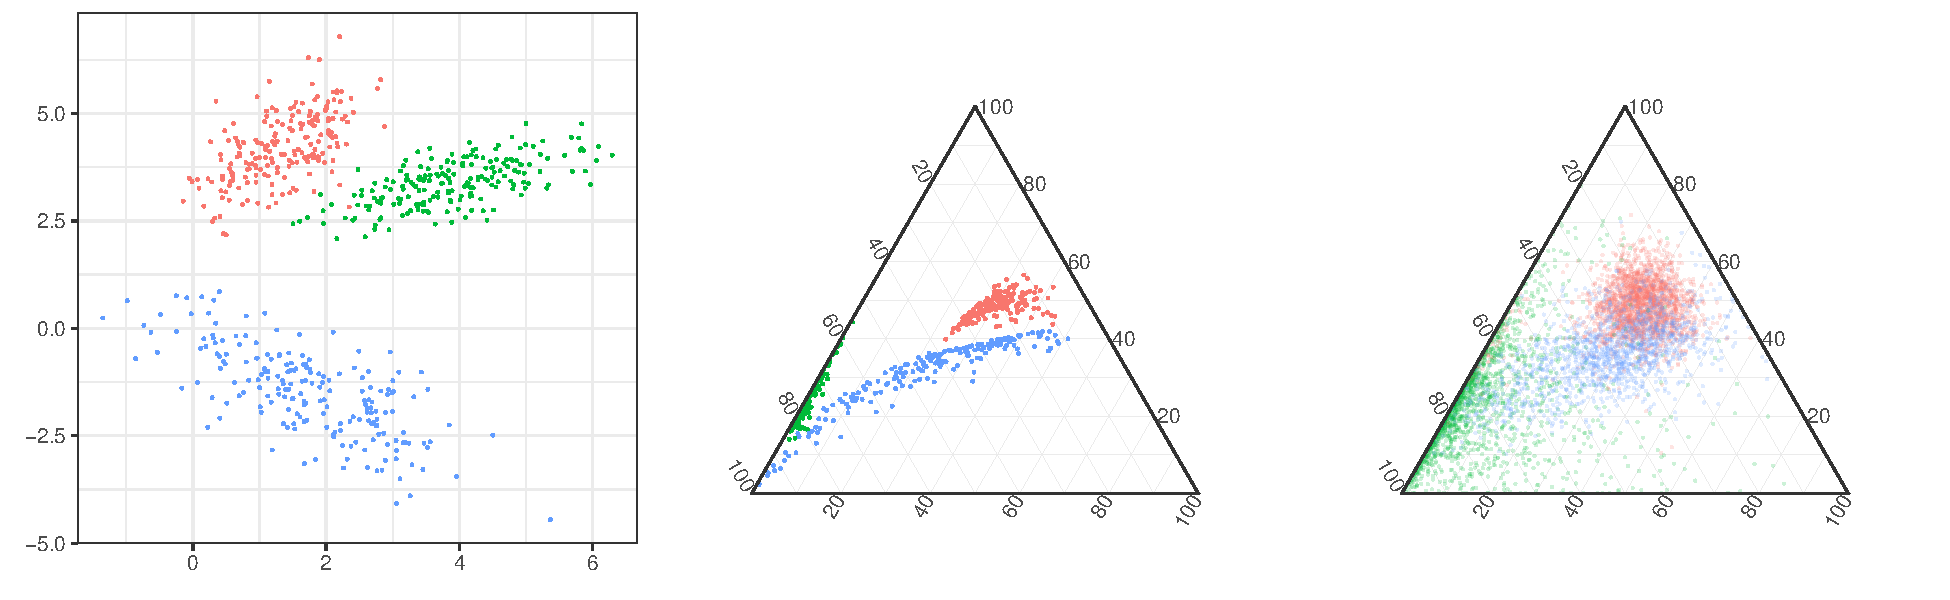
\includegraphics[width = \textwidth]{plots/simulated_reg}
\end{figure}















The term $\bm{x}_i$ is overloaded.  For $\bm{y}_{is}$ ($i$th observation, $s$th location), 
    $\bm{x}_{is}$ (covariates associated with observation $i$ at location $s$) include 
    $\bm{x}_{i,\text{obs}}$, the parameters under which the $i$th storm 
    was modelled; $\bm{x}_{s,\text{loc}}$, information pertaining to the $s$th location, such
    as latitude and longitude; and $\bm{x}_{is,\text{int}}$, any interaction thereof.  Currently
    this consists of a single term, the linear interaction between latitude of storm eye at landfall, 
    and latitude of location.




















% EOF